\subsection{Summary View}
\label{sec:allPairs}
Since we can only focus on one individual example at a time for detail analysis, how to pick a single pair of sentence from the development or test dataset (for the SNLI dataset, each of the these set consists of close to $10k$ examples) is an obvious challenge.
%
Beside the selection task, generate visual summarization there we also want to obtain certain high-level understand of how the whole set behave, beyond the information the prediction accuracy provide.

%treemap for prediction
As illustrate in Fig.~\ref{fig:summaryView}, we utilized a treemap (a) to encode the ground truth label and the model prediction generated by the
By click on the treemap cell, we can narrow down the selection by focus on specific senarios.


\begin{figure}[htbp]
\centering
\vspace{-2mm}
 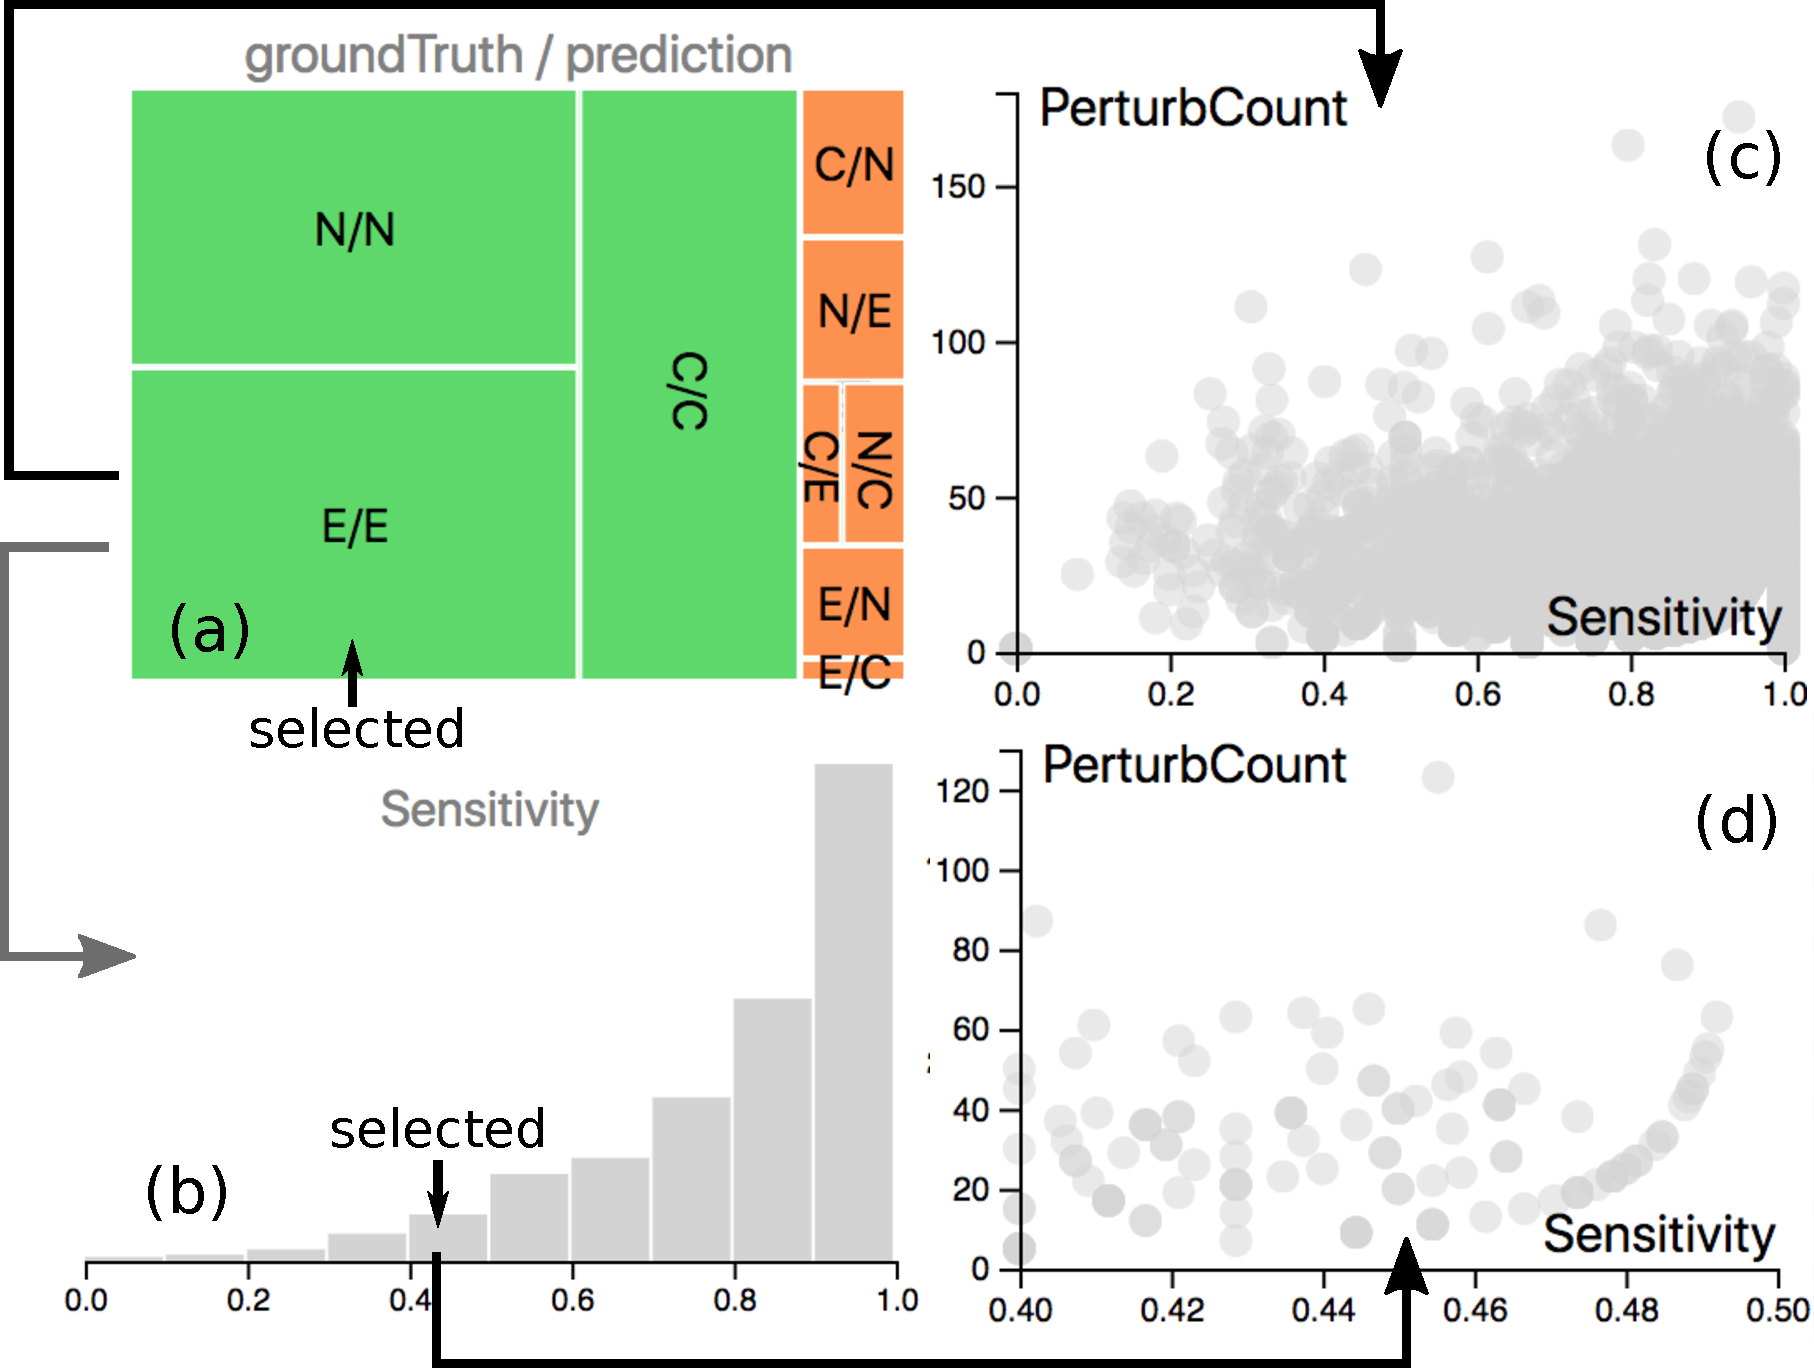
\includegraphics[width=1.0\linewidth]{summaryView}
 \caption{
Summarize the prediction results and sensitivity of the entire development set, and provide an explorative interface to select example of interests.
We summarize all the prediction results in (a), where the green block indicates correct predictions, and orange block indicates wrong predictions, and the label (e.g., E/E, E/N) indicates the ground truth label and the predicted label (N-Neural, E-Entailment, C-Contradiction).
%
The user can select the treemap to focus on the specific type of senarios and reveal the histogram (b) and scatterplot (c) for displaying per-pair information on the selected subset.
The selection can be further narrowed down by select the bin in the histogram.
In (c) and (d), each point corresponds to one prediction.
 }
\label{fig:summaryView}
\end{figure}

%The all pair
% \begin{itemize}
% \item How to go from 10k pair to one pair
% \item What constitute interesting example
% \item How to get a sense of overall prediction result
% \end{itemize}
